\section{Introduction}
\label{sec:-intro}

It is popular to model education as a process of ever-increasing 
specialization.  Preschool acclimatizes larval humans to basic 
scholarly etiquette (listening, sharing, naptime), while Kindergarten 
begins a focus on more distinct and practical skills such as reading, 
writing, and simple arithmetic.  high-school allows one to select a few 
electives, and the undergraduate degree program finally allows for the 
selection of the glorious Major.  By the time one has reached the PhD 
program, one's course of study has narrowed down to a mere fraction of 
the breadth of earlier, sometimes a single problem.

When dealing with questions on the frontiers of science, one sometimes 
encounters a number of subproblems that fall within the purview of many 
such narrow fields.  You start adding expert after expert to the team 
until you've got a 2-foot organizational chart and a half dozen 
management types trying to tell everyone what to do.  Interdisciplinary 
research doesn't seem to scale very well.

One of the real draws for machine learning lies in allowing us to 
compartmentalize our need for understanding.  So long as our model 
``understands'' a problem, we can ignore a certain level of complexity 
and move on to the interesting part.  This lets a computer scientist 
with a remarkable aversion to even thinking too deeply about the 
outdoors make a number of staggeringly correct judgemnts about forests, 
all from the comfort of their office.

We know a few things about a bit of forest, and an accomplished expert 
in the fields of ecology or geography, specializing in the climate of 
that forest, might be able to tell us quite a bit of information based 
on that starting data.  In the noble tradition of computer science, we 
would like to avoid doing that much work, and we will apply machine 
learning techniques to accomplish this task.  To that end, we consider 
the following multiclass classification problem. We construct a 
classifier that, when presented with a number of cartographic variables 
that apply to a 30--30 meter cell of forest, classifies such a cell by 
the predominant type of tree cover found therein.

We are presented with a collection of cartographic variables as 
enumerated in table \ref{table:featurelist}.  Some of 
these variables are continuous, as displayed in Figure 
\ref{fig:continuous_features}.  Others are lists of binary features 
designed to account for multiclass features in the one-hot encoding 
style, as observed in figures \ref{fig:soil} and \ref{fig:wilderness}.


\begin{figure*}
\centering
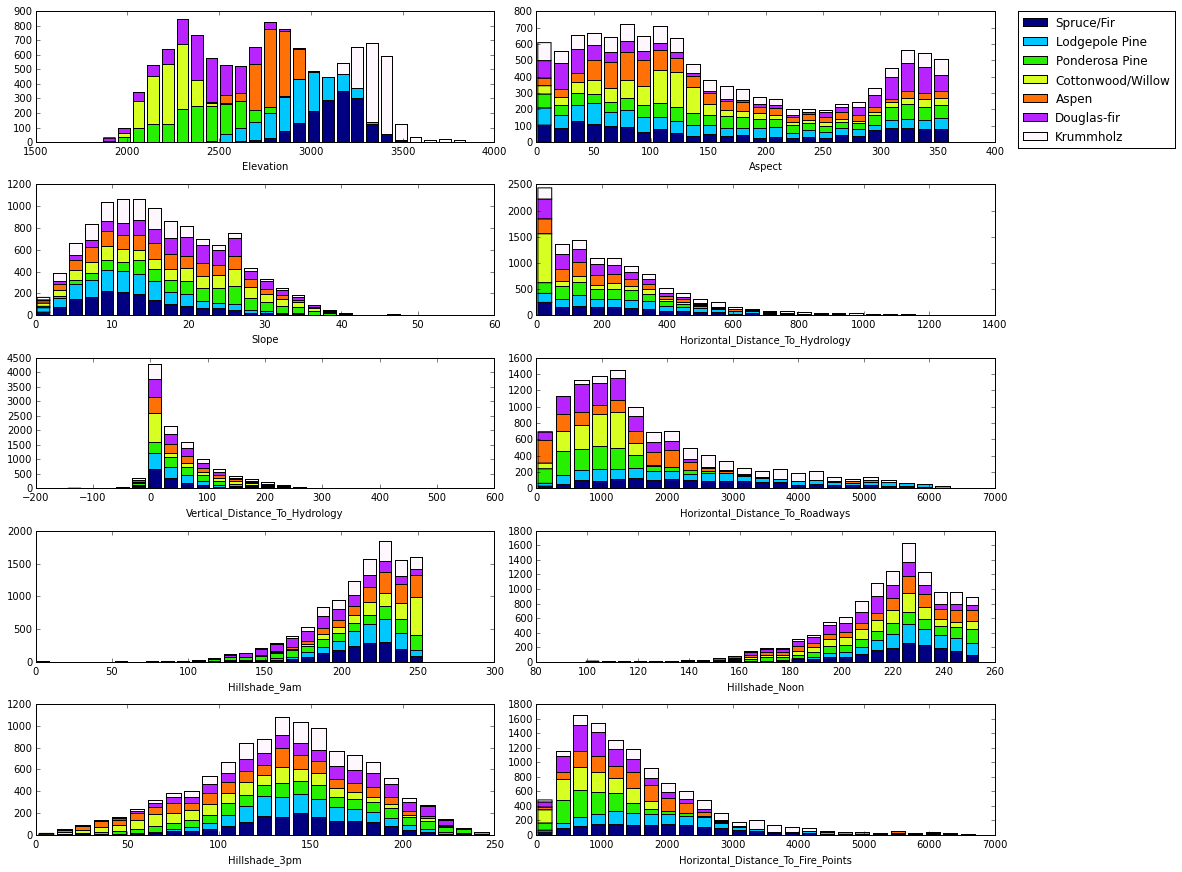
\includegraphics[width=\linewidth]{continuous}
 \caption{Continuous variables}
 \label{fig:continuous_features}
\end{figure*}

\begin{figure*}
\centering
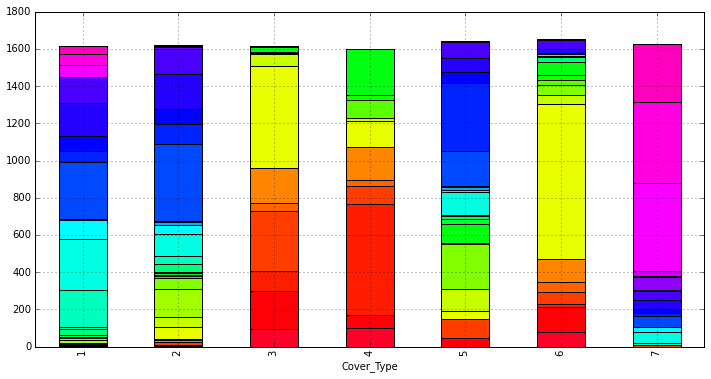
\includegraphics[width=\linewidth]{soil_type}
 \caption{Soil types and accompanying cover types}
 \label{fig:soil}
\end{figure*}

\begin{figure*}
\centering
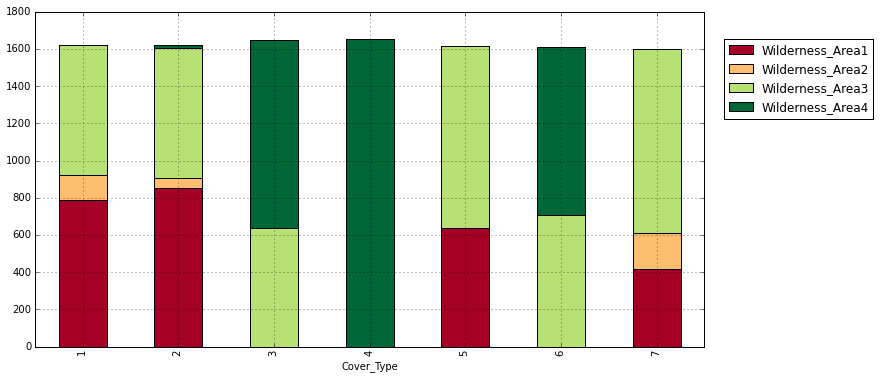
\includegraphics[width=\linewidth]{wilderness}
 \caption{Wilderness types and accompanying cover types}
 \label{fig:wilderness}
\end{figure*}


\begin{table}
  \begin{tabular}{ l | r }
    \hline
    Elevation & Elevation in meters \\
    \hline
    Aspect & Aspect in degrees azimuth \\
    \hline
    Slope & Slope in degrees \\
    \hline
    Horizontal\_Distance\_To\_Hydrology & Meters to nearest water-body \\
    \hline
    Vertical\_Distance\_To\_Hydrology & Meters to nearest water-body \\
    \hline
    Horizontal\_Distance\_To\_Roadways & Meters to nearest roadway \\
    \hline
    Hillshade\_9am (0 to 255 index) & Hillshade index at 9am \\
    \hline
    Hillshade\_Noon (0 to 255 index) & Hillshade index at noon \\
    \hline
    Hillshade\_3pm (0 to 255 index) & Hillshade index at 3pm \\
    \hline
    Horizontal\_Distance\_To\_Fire\_Points & Meters, wildfire ignition points \\
    \hline
    Wilderness\_Area & Wilderness area designation \\
    \hline
    Soil\_Type & Soil Type designation \\
    \hline
  \end{tabular}
  \caption{Feature List}
  \label{table:featurelist}
\end{table}


%%% Local Variables: 
%%% mode: latex
%%% TeX-master: "main"
%%% End: 
